{
\abnormalparskip{0pt}
\chapter{Experiments}
\label{cha:experiments}
}

Introduction, max 1/2--1 page

Naming of methods:
\begin{table}[htbp]
  \centering
  \begin{tabular}{cp{9cm}}
    \toprule
    Method       & Description                                      \\
    \midrule
    Simple       & New implementation with the analytical method.   \\
    SimpleSort   & New implementation with the analytical method and sorted
                   terminals.                                       \\
    SmithNew     & New implementation with \citeauthor{smith1992}'s
                   iteration.                                       \\
    SmithNewSort & New implementation with \citeauthor{smith1992}'s iteration
                   and sorted terminals.                            \\
    SmithOld     & Original implementation by \textcite{smith1992}. \\
    \bottomrule
  \end{tabular}
  \caption[Here be dragons]{Here be dragons.\label{tab:method-names}}
\end{table}

\section{Correctness}
\label{sec:correctness}

$150$ random cubes with $n = 10 \ldots 12$ and $d = 2$.

Simple seems faulty in a few instances:

Here it has a Steiner point lying atop another which in
smiths has been moved out from it a bit. Thus it seems the new iteration has
some situations with the error which it does not catch but is caugth by smiths
perturbations

\begin{table}[htbp]
  \centering
  \begin{tabular}{ccc}
    \toprule
    Instance           & Method     & Diff        \\
    \midrule
    cube\_n12\_d2\_s27 & Simple     & $0.0032114$ \\
    cube\_n12\_d2\_s49 & Simple     & $0.0062502$ \\
    cube\_n10\_d2\_s42 & SimpleSort & $0.0002782$ \\
    cube\_n12\_d2\_s26 & SimpleSort & $0.0040131$ \\
    cube\_n12\_d2\_s43 & SimpleSort & $0.0065104$ \\
    cube\_n12\_d2\_s49 & SimpleSort & $0.0062502$ \\
    \bottomrule
  \end{tabular}
  \caption[Here be dragons]{Here be dragons.\label{tab:correctness-errors}}
\end{table}

\section{Speed}
\label{sec:speed}

\begin{table}[htbp]
  \centering
  \begin{tabular}{ccccc}
    \toprule
    Set     & Dimensions       & Terminals             & Set size & Point configuration \\
    \midrule
    Carioca & $d = 3 \ldots 5$ & $n = 11 \ldots 16$    & $90$       & Random in cube      \\
    Cube    & $d = 2 \ldots 4$ & $n = 10 \ldots 15$    & $360$      & Random in cube      \\
    Iowa05  & $d = 3 \ldots 5$ & $n = 10$              & $30$       & Random in cube      \\
    Sausage & $d = 2 \ldots 5$ & $n = 10 \ldots 15$    & $24$       & Simplex sequence    \\
    Solids  & $d = 3$          & $n = 4, 6, 8, 12, 20$ & $5$        & Platonic solids     \\
    \bottomrule
  \end{tabular}
  \caption[Here be dragons]{Here be dragons.\label{tab:test-sets}}
\end{table}

\begin{table}[htbp]
  \centering
  \begin{tabular}{cccccc}
    \toprule
            & \multicolumn{5}{c}{Method}                               \\
    \cmidrule(l){2-6}
    Set     & Simple & SimpleSort & SmithNew & SmithNewSort & SmithOld \\
    \cmidrule(r){1-1}\cmidrule(l){2-6}
    Carioca & $81$   & $89$       & $73$     & $87$         & $76$     \\
    Cube    & $360$  & $360$      & $352$    & $360$        & $356$    \\
    Iowa05  & $30$   & $30$       & $30$     & $30$         & $30$     \\
    Sausage & $22$   & $23$       & $18$     & $22$         & $21$     \\
    Solids  & $4$    & $4$        & $4$      & $4$          & $4$      \\
    \bottomrule
  \end{tabular}
  \caption[Here be dragons]{Here be dragons.\label{tab:set-success}}
\end{table}

All sets have been taken from \textcite{fonseca2014}, but the sets Carioca and
Cube has been pruned.

8 $\times$ Intel\textsuperscript{\textregistered}
Xeon\textsuperscript{\textregistered} CPU E5-2630L @ 2.00 GHz and 16 GB RAM

Describe why I have pruned Carioca and Cube.

Plot all five against each other on interesting sets

\begin{figure}[htbp]
  \centering
  \begin{subfigure}[t]{0.5\textwidth}
    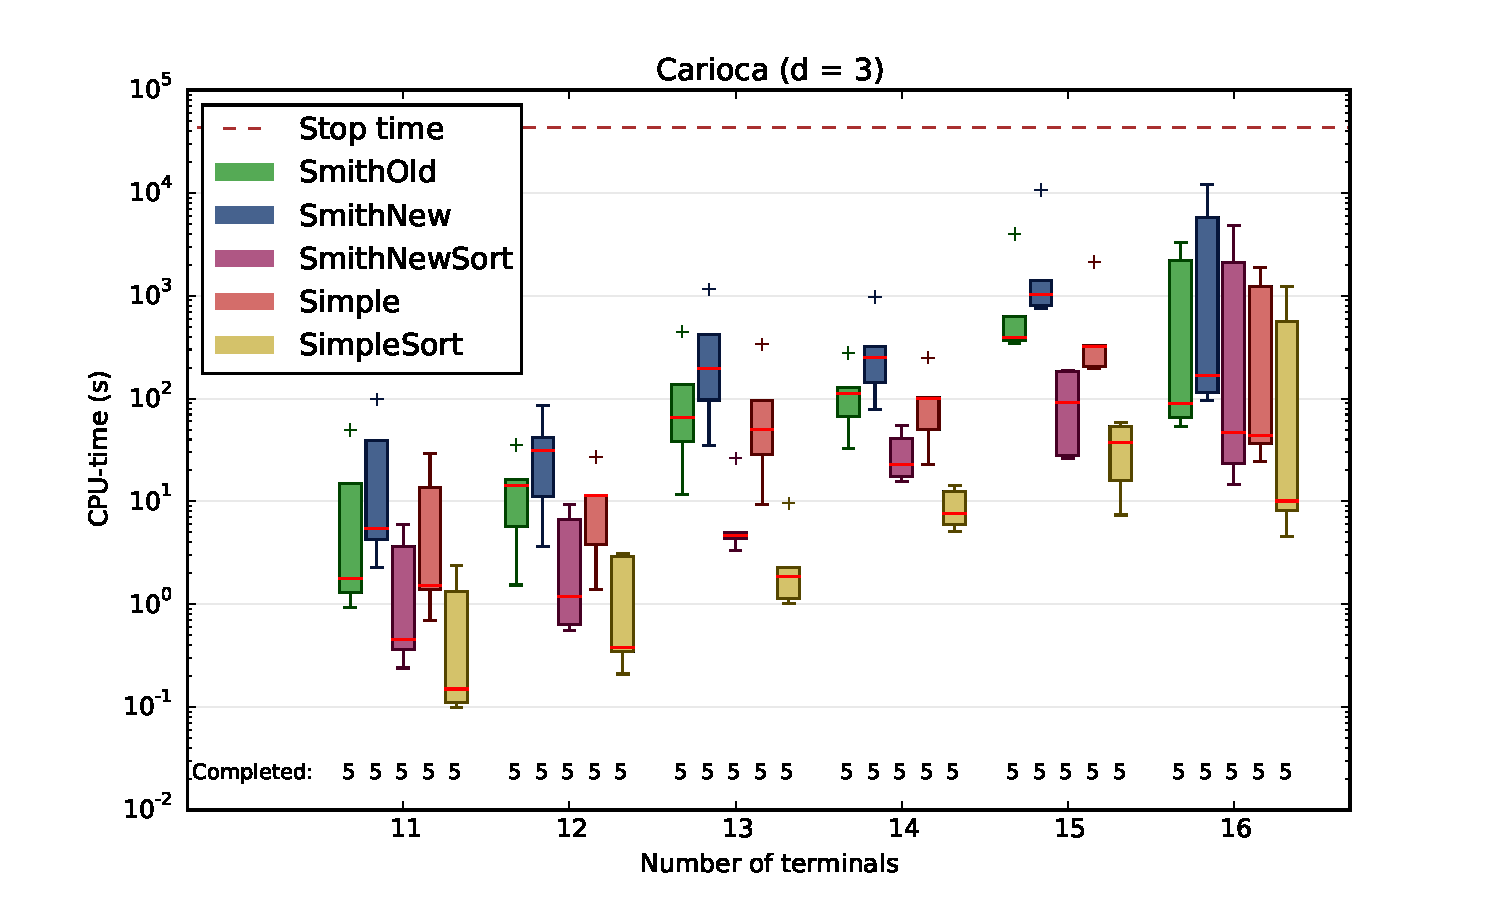
\includegraphics[width=\textwidth]{gfx/boxplots/plot_nvst_boxplot_d3_Carioca_1}
  \caption{Here be dragons.\label{fig:boxplot-d3-carioca-1}}
  \end{subfigure}%
  \begin{subfigure}[t]{0.5\textwidth}
    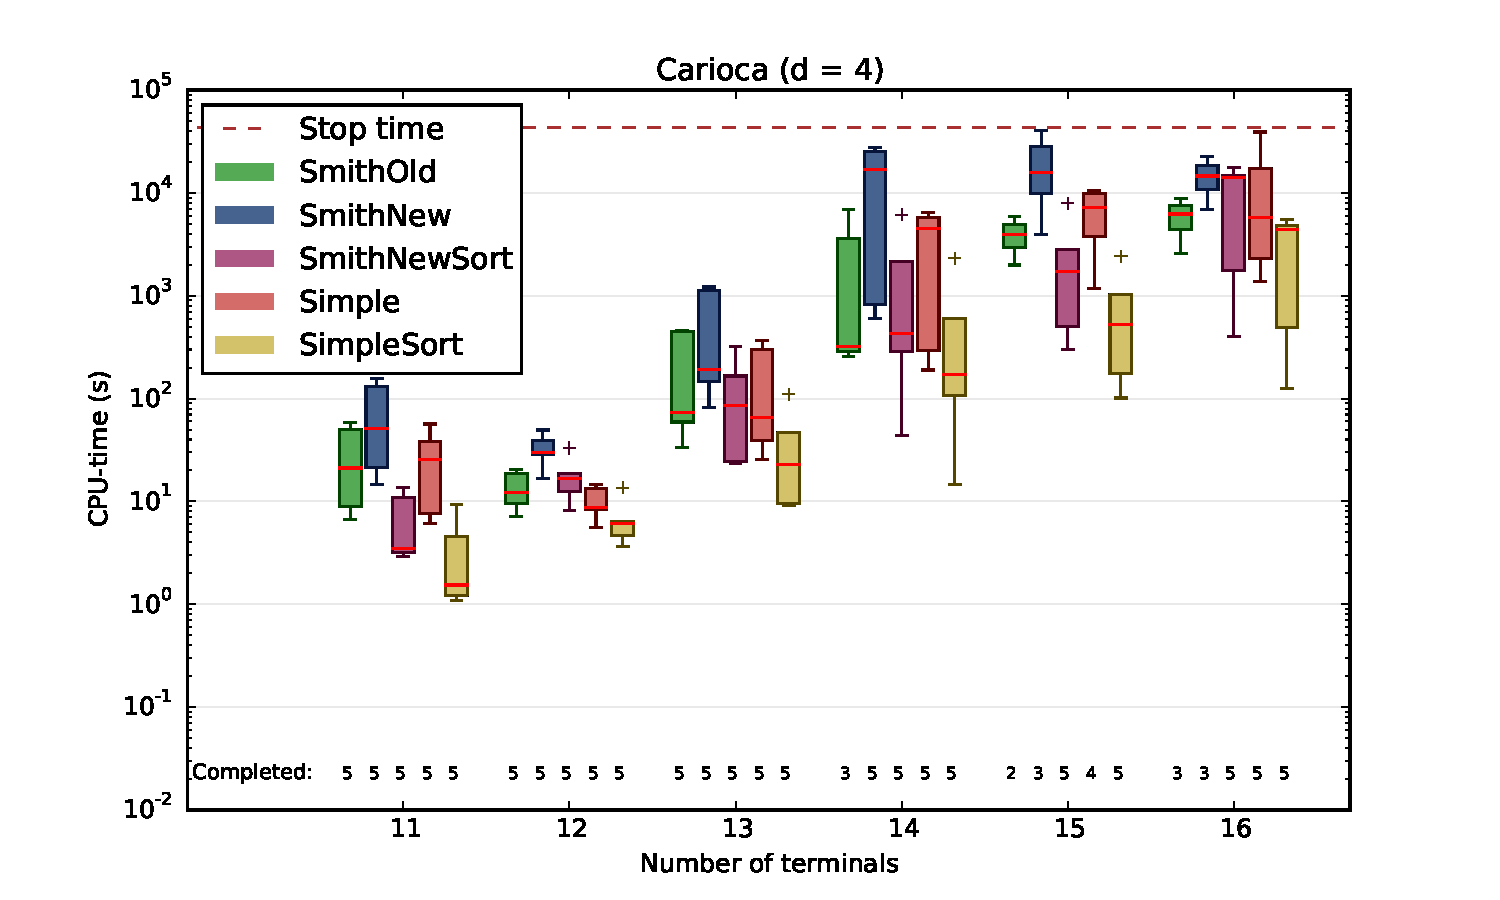
\includegraphics[width=\textwidth]{gfx/boxplots/plot_nvst_boxplot_d4_Carioca_1}
  \caption{Here be dragons.\label{fig:boxplot-d3-carioca-1}}
  \end{subfigure}%
  \caption[Here be dragons]{Here be dragons\label{fig:boxplot-carioca-1}}
\end{figure}

\begin{figure}[htbp]
  \centering
  \begin{subfigure}[t]{0.5\textwidth}
    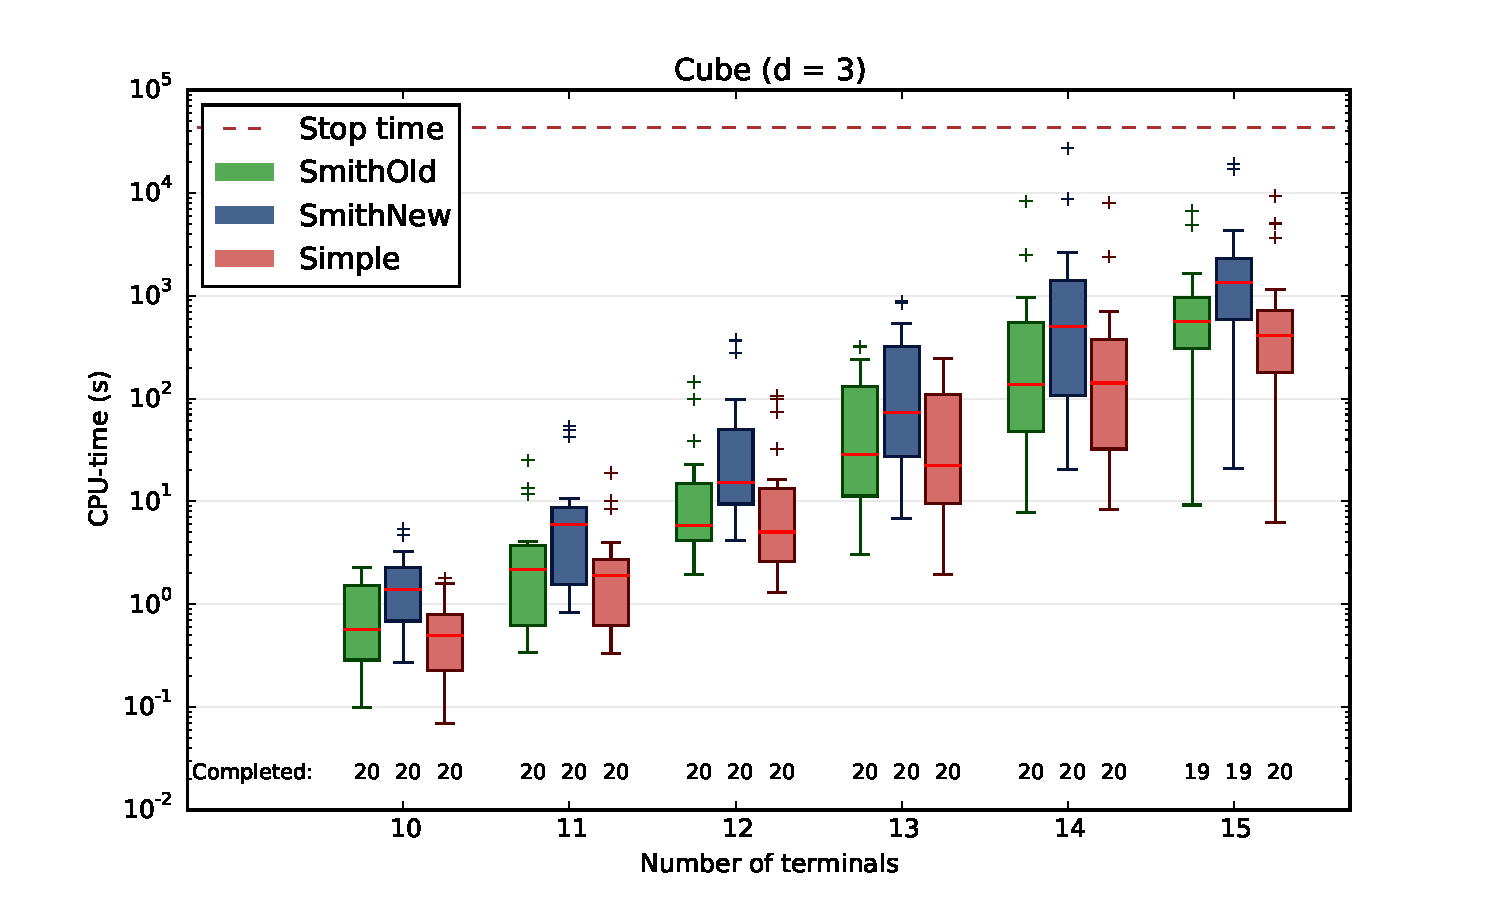
\includegraphics[width=\textwidth]{gfx/boxplots/plot_nvst_boxplot_d3_Cube_1}
  \caption{Here be dragons.\label{fig:boxplot-d3-cube-1}}
  \end{subfigure}%
  \begin{subfigure}[t]{0.5\textwidth}
    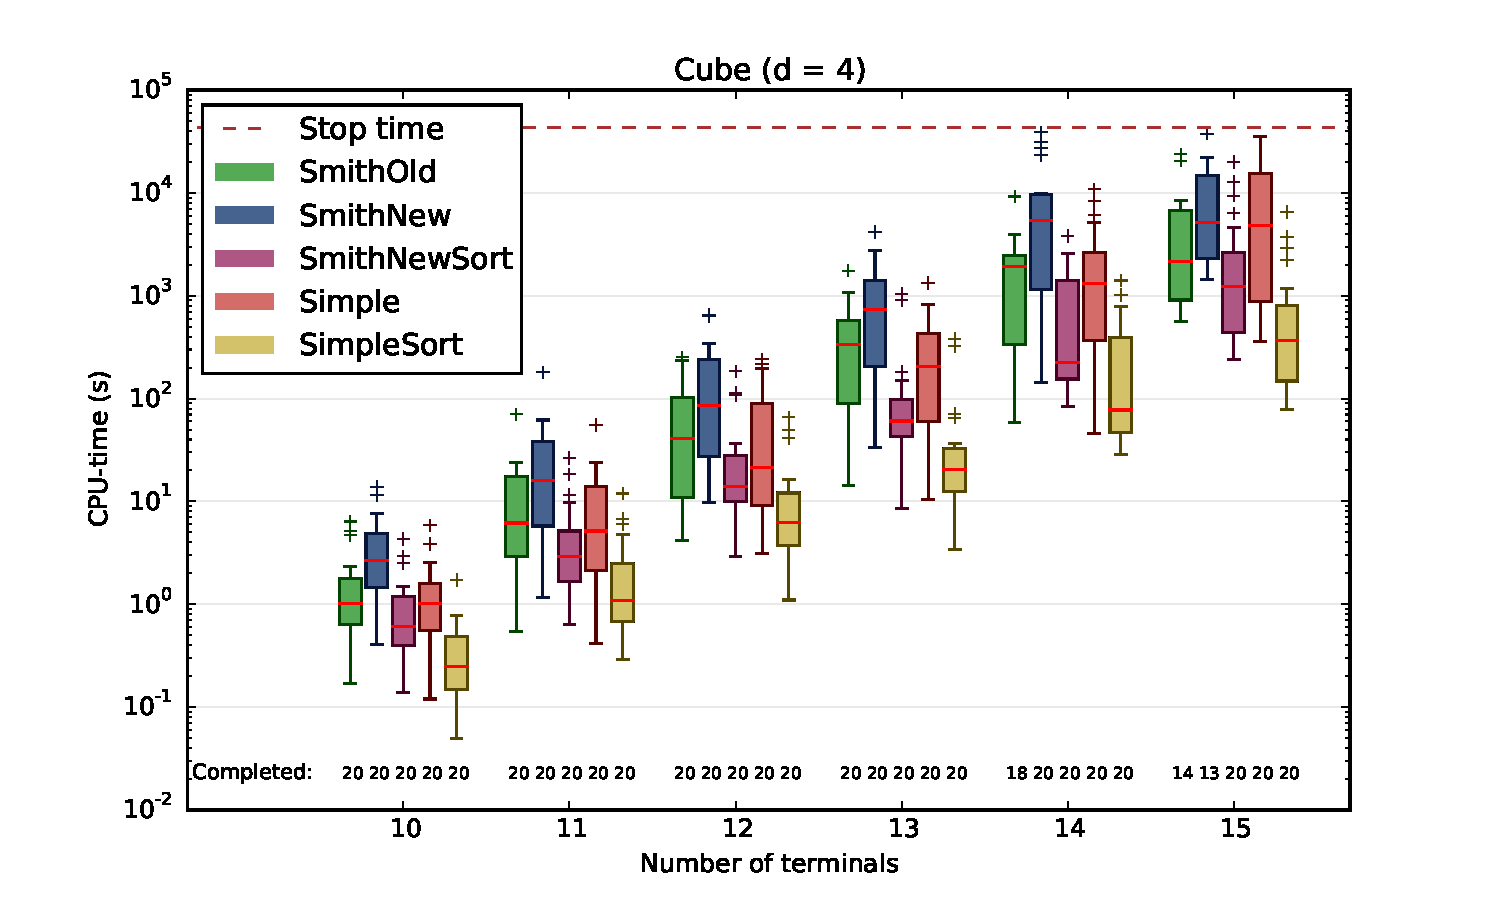
\includegraphics[width=\textwidth]{gfx/boxplots/plot_nvst_boxplot_d4_Cube_1}
  \caption{Here be dragons.\label{fig:boxplot-d3-cube-1}}
  \end{subfigure}%
  \caption[Here be dragons]{Here be dragons\label{fig:boxplot-cube-1}}
\end{figure}

\begin{figure}[htbp]
  \centering
  \begin{subfigure}[t]{0.5\textwidth}
    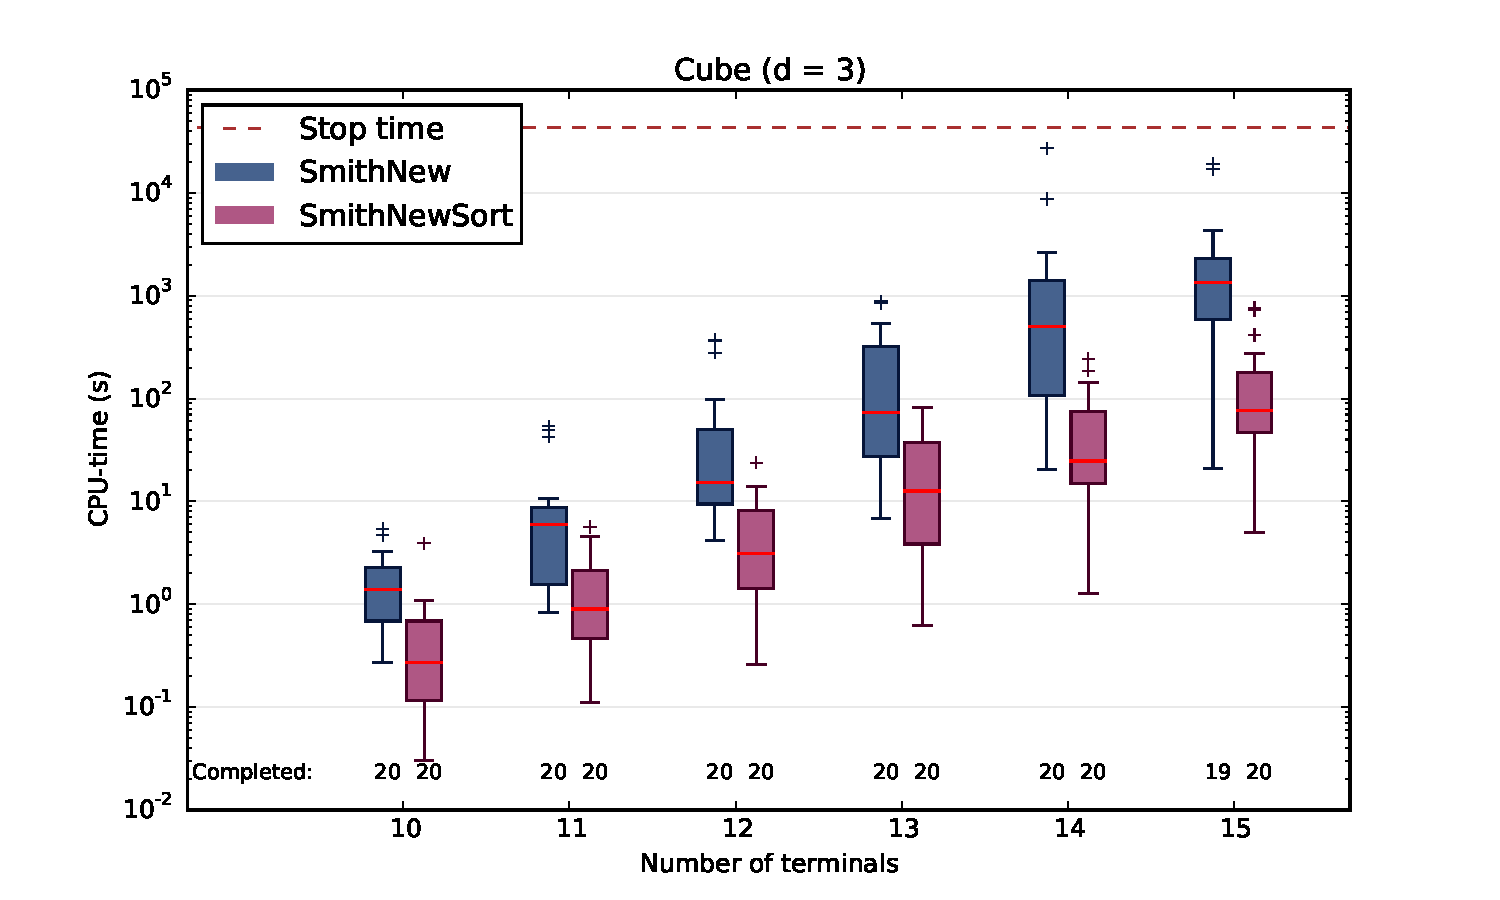
\includegraphics[width=\textwidth]{gfx/boxplots/plot_nvst_boxplot_d3_Cube_2}
  \caption{Here be dragons.\label{fig:boxplot-d3-cube-2}}
  \end{subfigure}%
  \begin{subfigure}[t]{0.5\textwidth}
    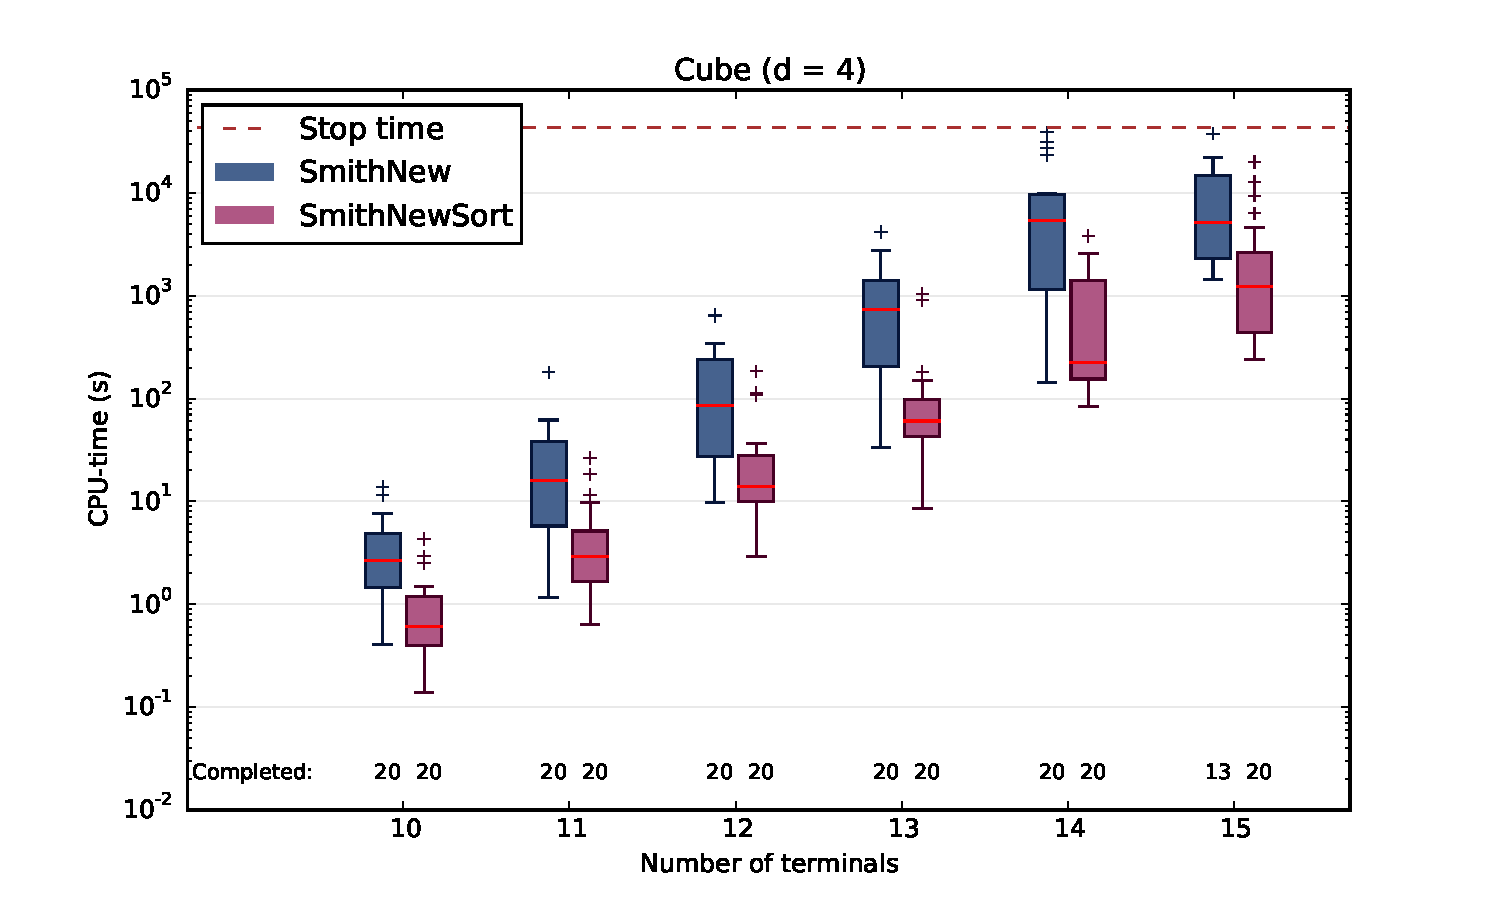
\includegraphics[width=\textwidth]{gfx/boxplots/plot_nvst_boxplot_d4_Cube_2}
  \caption{Here be dragons.\label{fig:boxplot-d3-cube-2}}
  \end{subfigure}%
  \caption[Here be dragons]{Here be dragons\label{fig:boxplot-cube-2}}
\end{figure}

\begin{figure}[htbp]
  \centering
  \begin{subfigure}[t]{0.5\textwidth}
    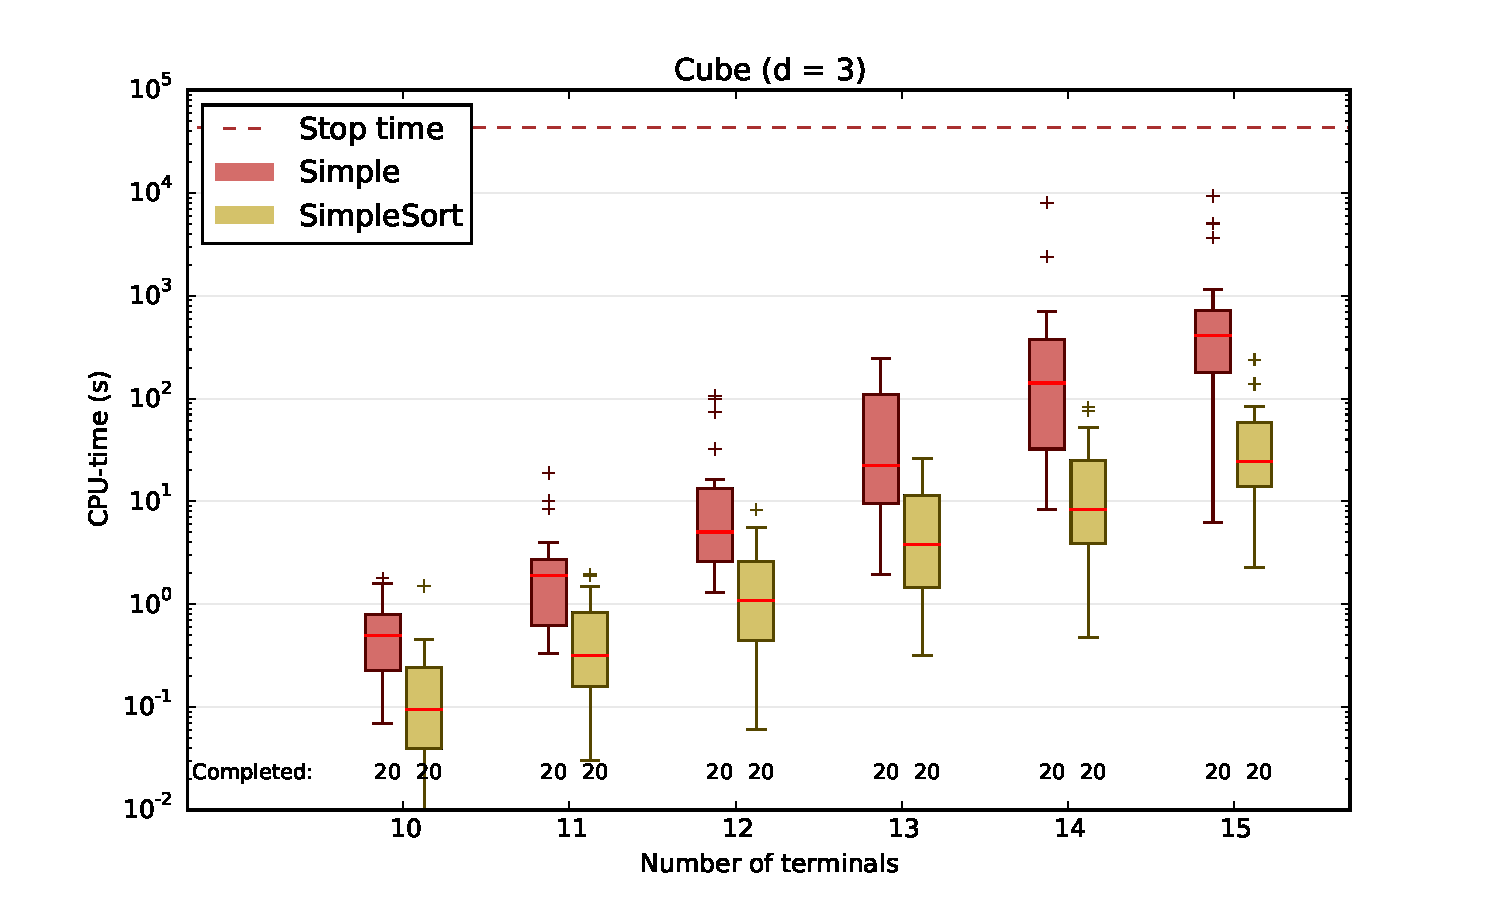
\includegraphics[width=\textwidth]{gfx/boxplots/plot_nvst_boxplot_d3_Cube_3}
  \caption{Here be dragons.\label{fig:boxplot-d3-cube-3}}
  \end{subfigure}%
  \begin{subfigure}[t]{0.5\textwidth}
    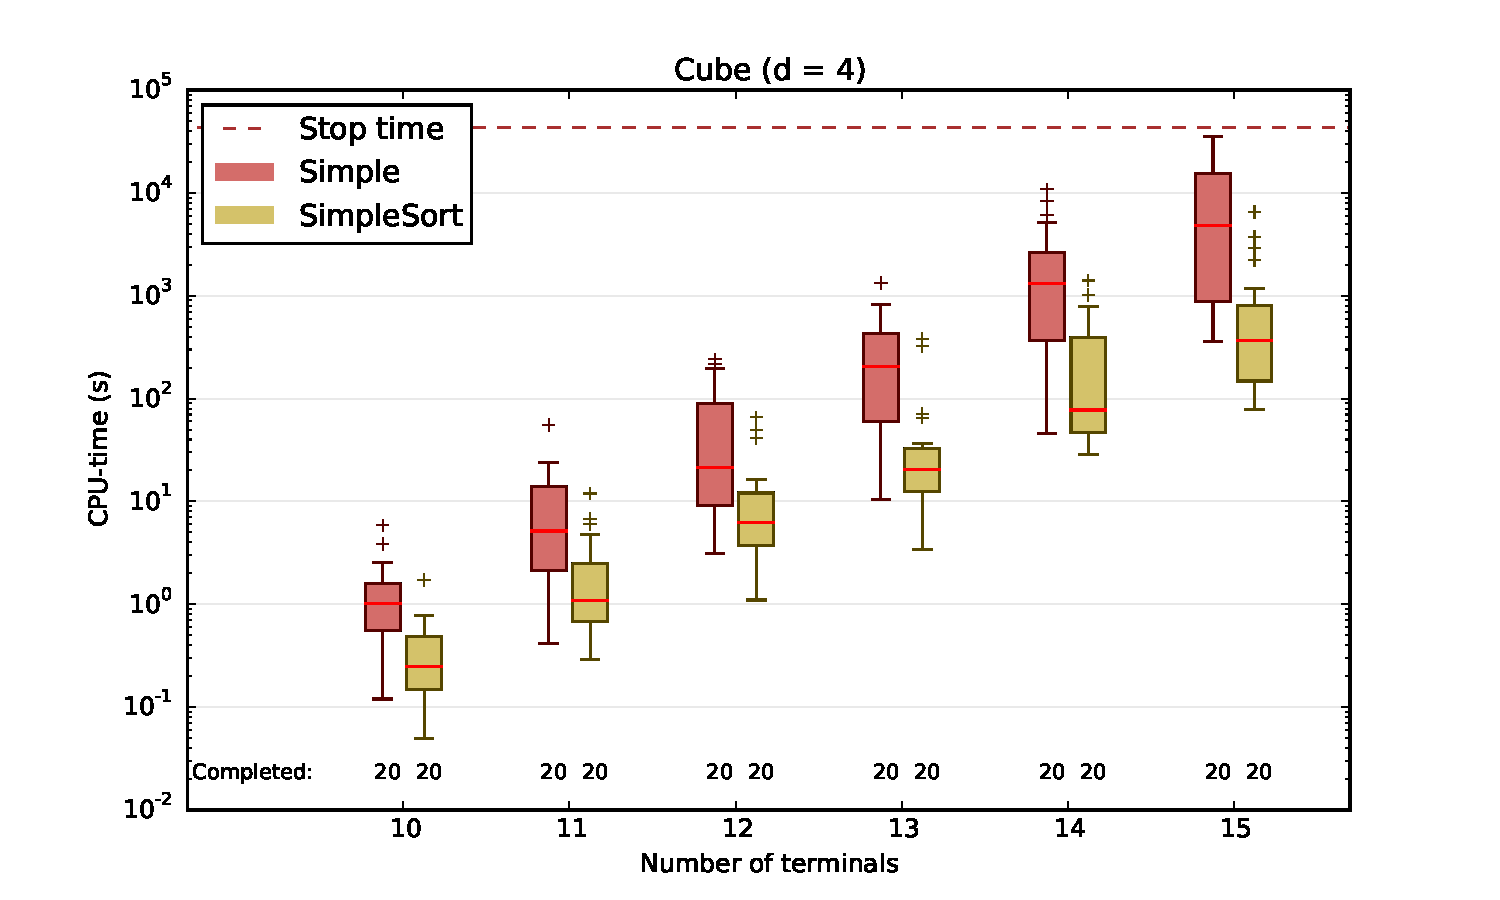
\includegraphics[width=\textwidth]{gfx/boxplots/plot_nvst_boxplot_d4_Cube_3}
  \caption{Here be dragons.\label{fig:boxplot-d3-cube-3}}
  \end{subfigure}%
  \caption[Here be dragons]{Here be dragons\label{fig:boxplot-cube-3}}
\end{figure}

\section{Trees and Iterations}
\label{sec:trees-iterations}

Introduction

\subsection{Trees}
\label{sec:trees}

\begin{table}[htbp]
  \centering
  \begin{tabular}{ccccccc}
    \toprule
         &     & \multicolumn{5}{c}{Method}                               \\
    \cmidrule(l){3-7}
    $n$  & $d$ & Simple & SimpleSort & SmithNew & SmithNewSort & SmithOld \\
    \cmidrule(r){1-2}\cmidrule(l){3-7}
    $10$ & $2$ & $1.04$ & $0.13$     & $1.42$   & $0.17$       & $1.00$   \\
         & $3$ & $1.21$ & $0.25$     & $1.70$   & $0.37$       & $1.00$   \\
         & $4$ & $1.17$ & $0.60$     & $1.61$   & $0.89$       & $1.00$   \\
         & $5$ & $1.54$ & $0.85$     & $2.25$   & $1.34$       & $1.00$   \\
    \cmidrule(r){1-2}
    $11$ & $2$ & $1.05$ & $0.10$     & $1.62$   & $0.13$       & $1.00$   \\
         & $3$ & $1.23$ & $0.19$     & $1.90$   & $0.29$       & $1.00$   \\
         & $4$ & $1.47$ & $0.36$     & $1.97$   & $0.56$       & $1.00$   \\
         & $5$ & $1.54$ & $0.77$     & $2.57$   & $1.22$       & $1.00$   \\
    \cmidrule(r){1-2}
    $12$ & $2$ & $1.17$ & $0.08$     & $1.90$   & $0.11$       & $1.00$   \\
         & $3$ & $1.42$ & $0.16$     & $2.34$   & $0.25$       & $1.00$   \\
         & $4$ & $1.73$ & $0.26$     & $2.83$   & $0.52$       & $1.00$   \\
         & $5$ & $1.53$ & $0.59$     & $2.24$   & $1.11$       & $1.00$   \\
    \cmidrule(r){1-2}
    $13$ & $2$ & $1.11$ & $0.05$     & $2.22$   & $0.09$       & $1.00$   \\
         & $3$ & $1.43$ & $0.12$     & $2.80$   & $0.20$       & $1.00$   \\
         & $4$ & $0.74$ & $0.25$     & $3.19$   & $0.43$       & $1.00$   \\
         & $5$ & $1.66$ & $0.45$     &          & $1.14$       & $1.00$   \\
    \cmidrule(r){1-2}
    $14$ & $2$ & $0.97$ & $0.05$     & $2.63$   & $0.08$       & $1.00$   \\
         & $3$ & $1.61$ & $0.10$     & $3.44$   & $0.19$       & $1.00$   \\
         & $4$ & $1.52$ & $0.16$     &          & $0.39$       & $1.00$   \\
         & $5$ &        &            &          &              &          \\
    \cmidrule(r){1-2}
    $15$ & $2$ & $1.32$ & $0.04$     & $3.12$   & $0.06$       & $1.00$   \\
         & $3$ &        &            &          &              &          \\
         & $4$ &        &            &          &              &          \\
         & $5$ &        &            &          &              &          \\
    \bottomrule
  \end{tabular}
  \caption[Here be dragons]{Here be dragons.\label{tab:trees-sausage}}
\end{table}

\subsection{Iterations}
\label{sec:iterations}

\begin{table}[htbp]
  \centering
  \small
  \begin{tabular}{cccccc}
    \toprule
         & \multicolumn{5}{c}{Method}                               \\
    \cmidrule(l){2-6}
    $n$  & Simple & SimpleSort & SmithNew & SmithNewSort & SmithOld \\
    \cmidrule(r){1-1}\cmidrule(l){2-6}
    $4$  & $0.24$ & $0.25$     & $0.99$   & $0.99$       & $1.00$   \\
    $6$  & $0.34$ & $0.33$     & $0.98$   & $1.01$       & $1.00$   \\
    $8$  & $0.28$ & $0.26$     & $1.38$   & $1.19$       & $1.00$   \\
    $12$ & $0.17$ & $0.12$     & $1.49$   & $1.51$       & $1.00$   \\
    $20$ &        &            &          &              &          \\
    \bottomrule
  \end{tabular}
  \caption[Here be dragons]{Here be dragons.\label{tab:iterations-solids-ratio}}
\end{table}

%%% Local Variables:
%%% mode: latex
%%% TeX-master: "../../main"
%%% End:
